\documentclass{bht-thesis}

\usepackage[ngerman]{babel}
\usepackage[utf8]{inputenc} % Required for inputting international characters
\usepackage[T1]{fontenc} % Output font encoding for international characters
\usepackage{mathpazo} % Use the Palatino font by default

\usepackage{blindtext}

% \usepackage[backend=bibtex,style=authoryear,natbib=true]{biblatex} % Use the bibtex backend with the authoryear citation style (which resembles APA)

% \addbibresource{example.bib} % The filename of the bibliography

% \usepackage[autostyle=true]{csquotes} % Required to generate language-dependent quotes in the bibliography

% Options for KOMA script scrrpt
\KOMAoptions{
	fontsize=11pt,
	paper=a4,
	DIV=calc,
	twoside=false,
	twocolumn=false,
	draft=false
	}
	
% Page settings
\geometry{
	% showframe,
	left=2.5cm,
	right=2.5cm,
	top=2.5cm,
	bottom=2.5cm
	}

% Information about the thesis
\title{Master Thesis}
\degree{Master of Science}
\university{Beuth Hochschule für Technik Berlin}
\faculty{Fachbereich VI - Informatik und Medien}
\course{Medieninformatik}

\thesistitle{Titel der Abschlussarbeit}
\author{Peter Pan}

\address{Bla Str. 123\\14852 Berlin}
\matnr{123456}
\phone{+49 1234 56789}
\email{peter@pan.de}
\city{Berlin}

\supervisor{Prof. Bla}
\expert{Prof. Blubb}


% Document starts here
\begin{document}
\cleardoublepage
\pagenumbering{Roman}
\maketitle
\tableofcontents
\listoffigures
\cleardoublepage
\pagenumbering{arabic}
\chapter{Einleitung}
\section{Jo}
\blindtext[4]
\section{Jojo}
\blindtext[2]
\section{Lala}
\blindtext[3]
\chapter{Fazit}
\section{Bla}
\blindtext[1]
\begin{figure}
	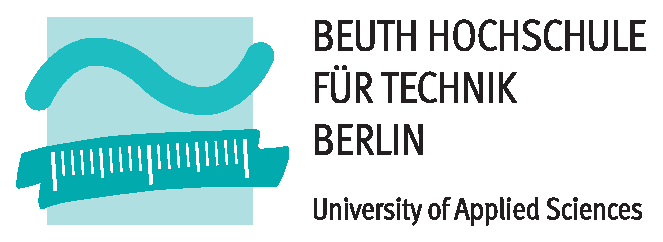
\includegraphics{figures/Beuth-Logo_basis}
	\centering
	\caption{Beuth Logo}
	\label{fig:bht-logo}
\end{figure}
\subsection{Blablubb}
\blindtext[4]
\end{document}